\appendix

\section{Evaluation of the redshift distribution}
\label{sec:moments}

Perhaps the most popular application of \pzpdf s is the estimation of the overall redshift distribution $N(z)$, a quantity that enters some cosmological calculations and the true value of which is known for the DC1 data set and will be denoted as $\tilde{N}(z)$.
In terms of the prior information provided to each method, the true redshift distribution satisfies the tautology $\tilde{N}(z) = p(z \vert I_{D})$ due to our experimental set-up; because the DC1 training and template sets are representative and complete, $I_{D}$ represents a prior that is also equal to the truth.
In this ideal case of complete and representative prior information, the method that would give the best approximation to $\hat{N}(z)$ would be one that neglects all the information contained in the photometry $\{d_{i}\}_{N_{tot}}$ and gives every galaxy the same \pzpdf\ $\hat{p}_{i}(z) = \tilde{N}(z)$ for all $i$; the inclusion of any information from the photometry would only introduce noise to the optimal result of returning the prior.
This is the exact estimator, \trainz, that we have described in Section~\ref{sec:trainz}, and which will serve as an experimental control.

\subsection{Metrics of the stacked estimator of the redshift distribution}
\label{sec:stackedmetrics}

``Stacking'' according to
\begin{equation}
  \label{eq:stacked}
  \hat{N}^{H}(z) \equiv \frac{1}{N_{tot}}\ \sum_{i}^{N_{tot}}\ \hat{p}^{H}_{i}(z)
\end{equation}
 is the most widely used method for obtaining $\hat{N}^{H}(z)$ as an estimator of the redshift distribution from \pzpdf s derived by a method $H$. While the stacked estimator of the redshift distribution violates the mathematical definition of statistical independence and is thus not formally correct\footnote{Malz \& Hogg (in prep) shows how the stacking procedure can lead to bias in the estimate of $N(z)$ and presents a principled alternative to this commonly employed method.  See \url{https://github.com/aimalz/chippr} for details.}, we use it as a basis for comparison of \pzpdf\ methods under the untested assumption that the response of our metrics of $\hat{N}^{H}(z)$ will be analogous to the same metrics applied to a principled estimator of the redshift distribution.


As $N(z)$ is itself a univariate PDF, we apply the metrics of the previous sections to it as well.
We additionaly calculate the first three moments
\begin{equation}
  \label{eq:moment}
  \langle z^{m}\rangle \equiv \int_{-\infty}^{\infty} z^{m} N(z) dz
\end{equation}
of the estimated redshift distribution $\hat{N}^{H}(z)$ for each code and compare them to the moments of the true redshift distribution $\tilde{N}(z)$.
Under the assumption that the stacked estimator is unbiased, a superior method minimizes the difference between the true and estimated moments.

\subsection{Performance on the stacked estimator of the redshift distribution}
\label{sec:stackedmetrics_results}

Figure~\ref{fig:nz} shows the stacked estimator $\hat{N}(z)$ of the redshift distribution for each code compared to the true redshift distribution $\tilde{N}(z)$, where the stacked estimator has been smoothed for each code in the plot using a kernel density estimate (KDE) with a bandwidth chosen by Scott's Rule \citep{Scott:1992} in order to minimize visual differences in small-scale features; the quantiative statistics, however, are calculated using the empirical CDF which is not smoothed.

\begin{figure*}
\centering
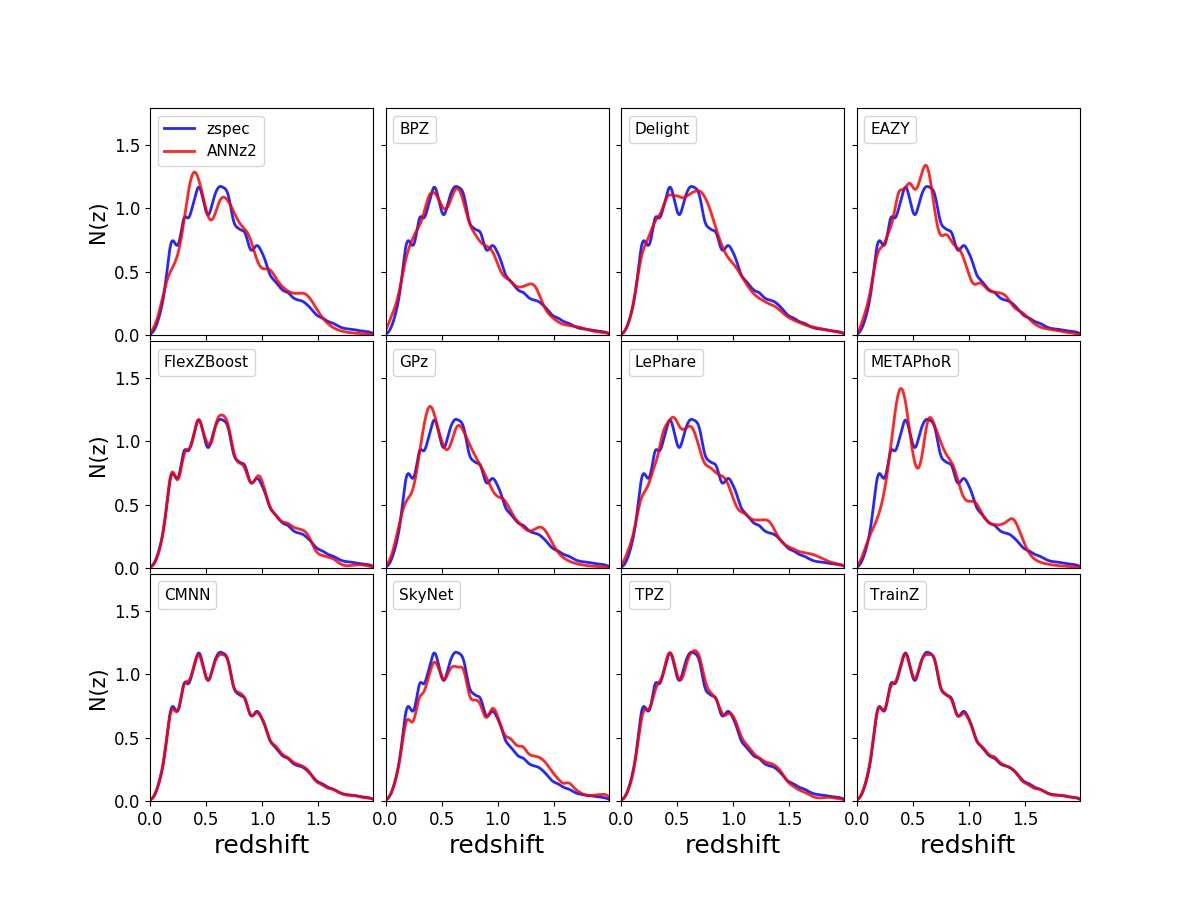
\includegraphics[width=0.74\textwidth]{fig/NZsumplot_12codes_scottsrule.jpg}
\caption{The smoothed stacked estimator $\hat{N}(z)$ of the redshift distribution (red) produced by each code (panels) compared to the true redshift distribution $\tilde{N}(z)$ (blue).
Varying levels of agreement are seen among the codes, with the smallest deviations for \cmnn, \flexzboost, \tpz, and \trainz.}
\label{fig:nz}
\end{figure*}

Many of the codes, including all the model-fitting approaches and \annz, \gpz, \metaphor, and \skynet\ from the data-driven camp, overestimate the redshift density at $z \sim 1.4$.
This behavior is a consequence of the $4000$ \AA\ break passing through the gap between the $z$ and $y$ filters, which induces a genuine discontinuity in the $z - y$ colour as a function of redshift that can sway the \pzpdf\ estimates in the absence of bluer spectral features.

\annz, \gpz, and \metaphor\ feature exaggerated peaks and troughs relative to the training set, a potential sign of overtraining.
Further investigation on overtraining is needed, if present this is an obstacle that may be overcome with adjustment of the implementation.

As expected, \trainz\ perfectly recovers the true redshift distribution: as the training sample is selected from the same underlying distribution as the test set, the redshift distributions are identical, up to Poisson fluctuations due to the finite number of sample galaxies.
\cmnn\ is also in excellent agreement for similar reasons: with a representative training sample of galaxies spanning the colour-space, the sum of the colour-matched neighbour redshifts should return the true redshift distribution.
\flexzboost\ and \tpz\ also perform superb recovery of the true redshift distribution, with only a slight deviation at $z \sim 1.4$.
Our metrics, however, cannot discern whether these four approaches, as well as \delight, are spared the $z \sim 1.4$ degeneracy in $\hat{N}(z)$ because they have more effectively used information in the data or if the impact is simply washed out by the stacked estimator's effective average over the test set galaxy sample.
See Appendix~\ref{sec:pointmetrics} for further discussion of the $z \sim 1.4$ issue.

Figure~\ref{fig:nz_stats} shows the quantitative Kolmogorov-Smirnoff (KS), Cramer-Von Mises (CvM), and Anderson Darling (AD) test statistics for each of the codes for the $\hat{N}(z)$ based measures.
The horizontal lines show the the result of a bootstrap resampling of the training set using 30,000 samples for \trainz, representing a conservative idealized limit on expected performance for a modest-sized representative training set of galaxies, as mentioned in Section~\ref{sec:pitqq}.
The AD bootstrap statistic is elevated due to its sensitivity to the tails of distributions.
The stacked estimators of the redshift distribution for \cmnn\ and \trainz\ best estimate $\tilde{N}(z)$ under these metrics, whereas \eazy, \lephare, \metaphor, and \skynet\ underperform; \bpz, \gpz, and \tpz\ are within a factor of two of the conservative limit for all statistics.
It is unsurprising that \cmnn\ scores well, as with a nearly complete and representative training set choosing neighbouring points in colour/magnitude space to construct an estimator should lead to excellent agreement in the final $\hat{N}(z)$.

\begin{figure*}
\centering
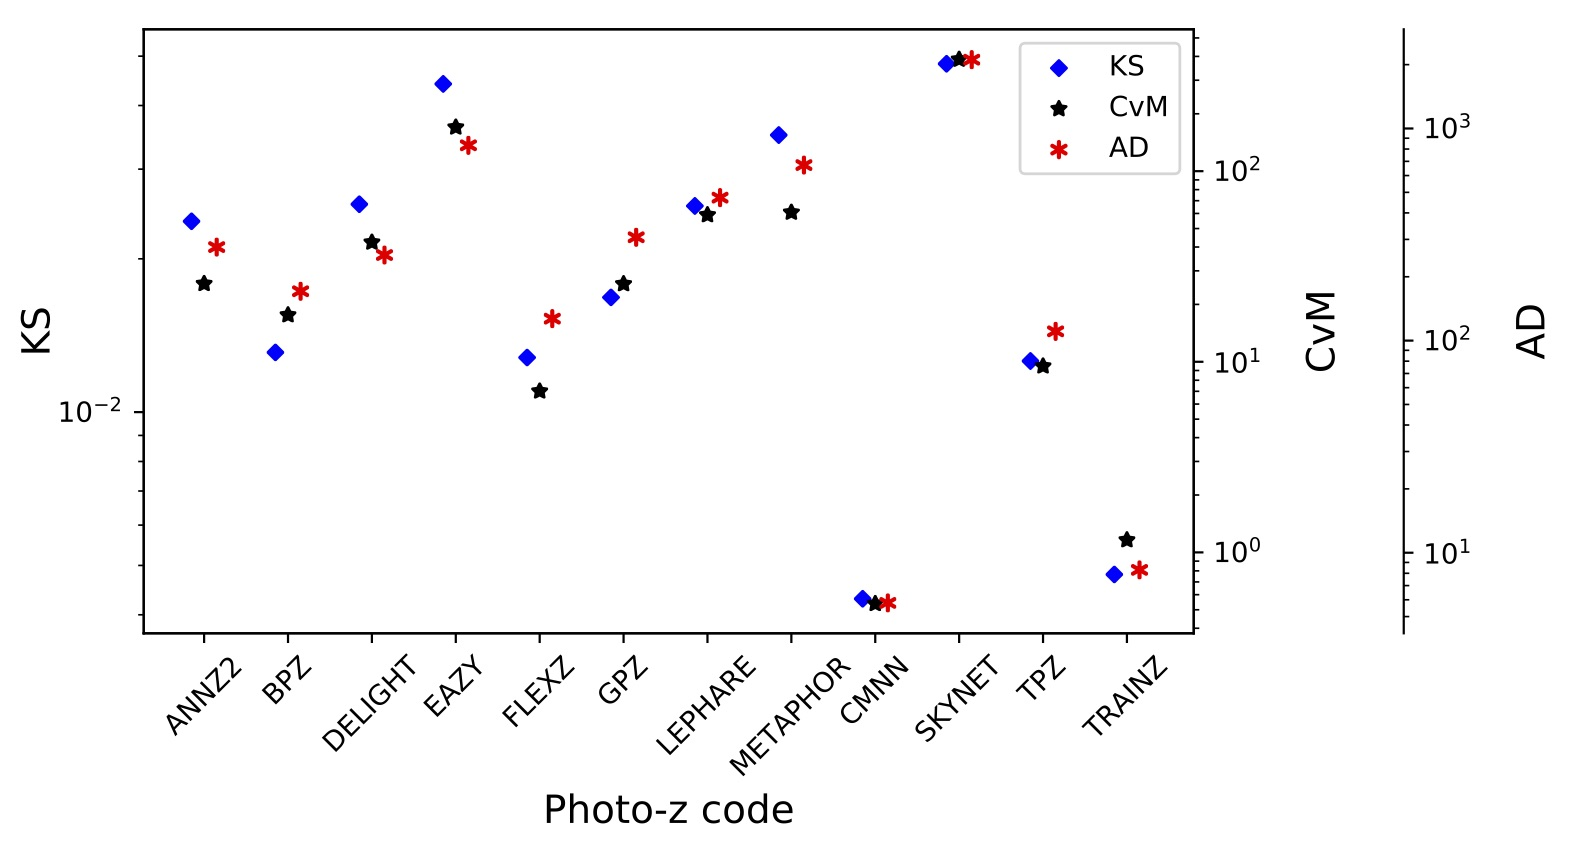
\includegraphics[width=0.74\textwidth]{fig/KSvsCvMvsAD_NZ_withnull_jpg.jpg}
\caption{A visualization of the Kolmogorov-Smirnoff (KS, blue diamond), Cramer-von Mises (CvM, black star), and Anderson-Darling (AD, red asterisk) statistics for the $\hat{N}(z)$ distributions.
Horizontal lines indicate the statistic values (including uncertainty) achieved using \trainz\ via bootstrap resampling a training set containing 30,000 redshifts.
We make the reassuring observation that these related statistics do not disagree significantly with one another.
\cmnn\ outperforms the control case, \trainz, and several codes are within a factor of two of this conservative idealized limit.
\skynet\ scores poorly due to an overall bias in its redshift predictions.}
\label{fig:nz_stats}
\end{figure*}

It is, however, surprising that \tpz\ does well on $\hat{N}(z)$ given its poor performance on the ensemble \pzpdf s, especially knowing that \tpz\ was optimized for \pzpdf\ ensemble metrics rather than the stacked estimator of the redshift distribution.
A possible explanation is the choice of smoothing parameter chosen during validation, which affects \pzpdf\ widths as well as overall redshift bias and could be modified to improve performance under the \pzpdf\ metrics.

\begin{figure*}
\centering
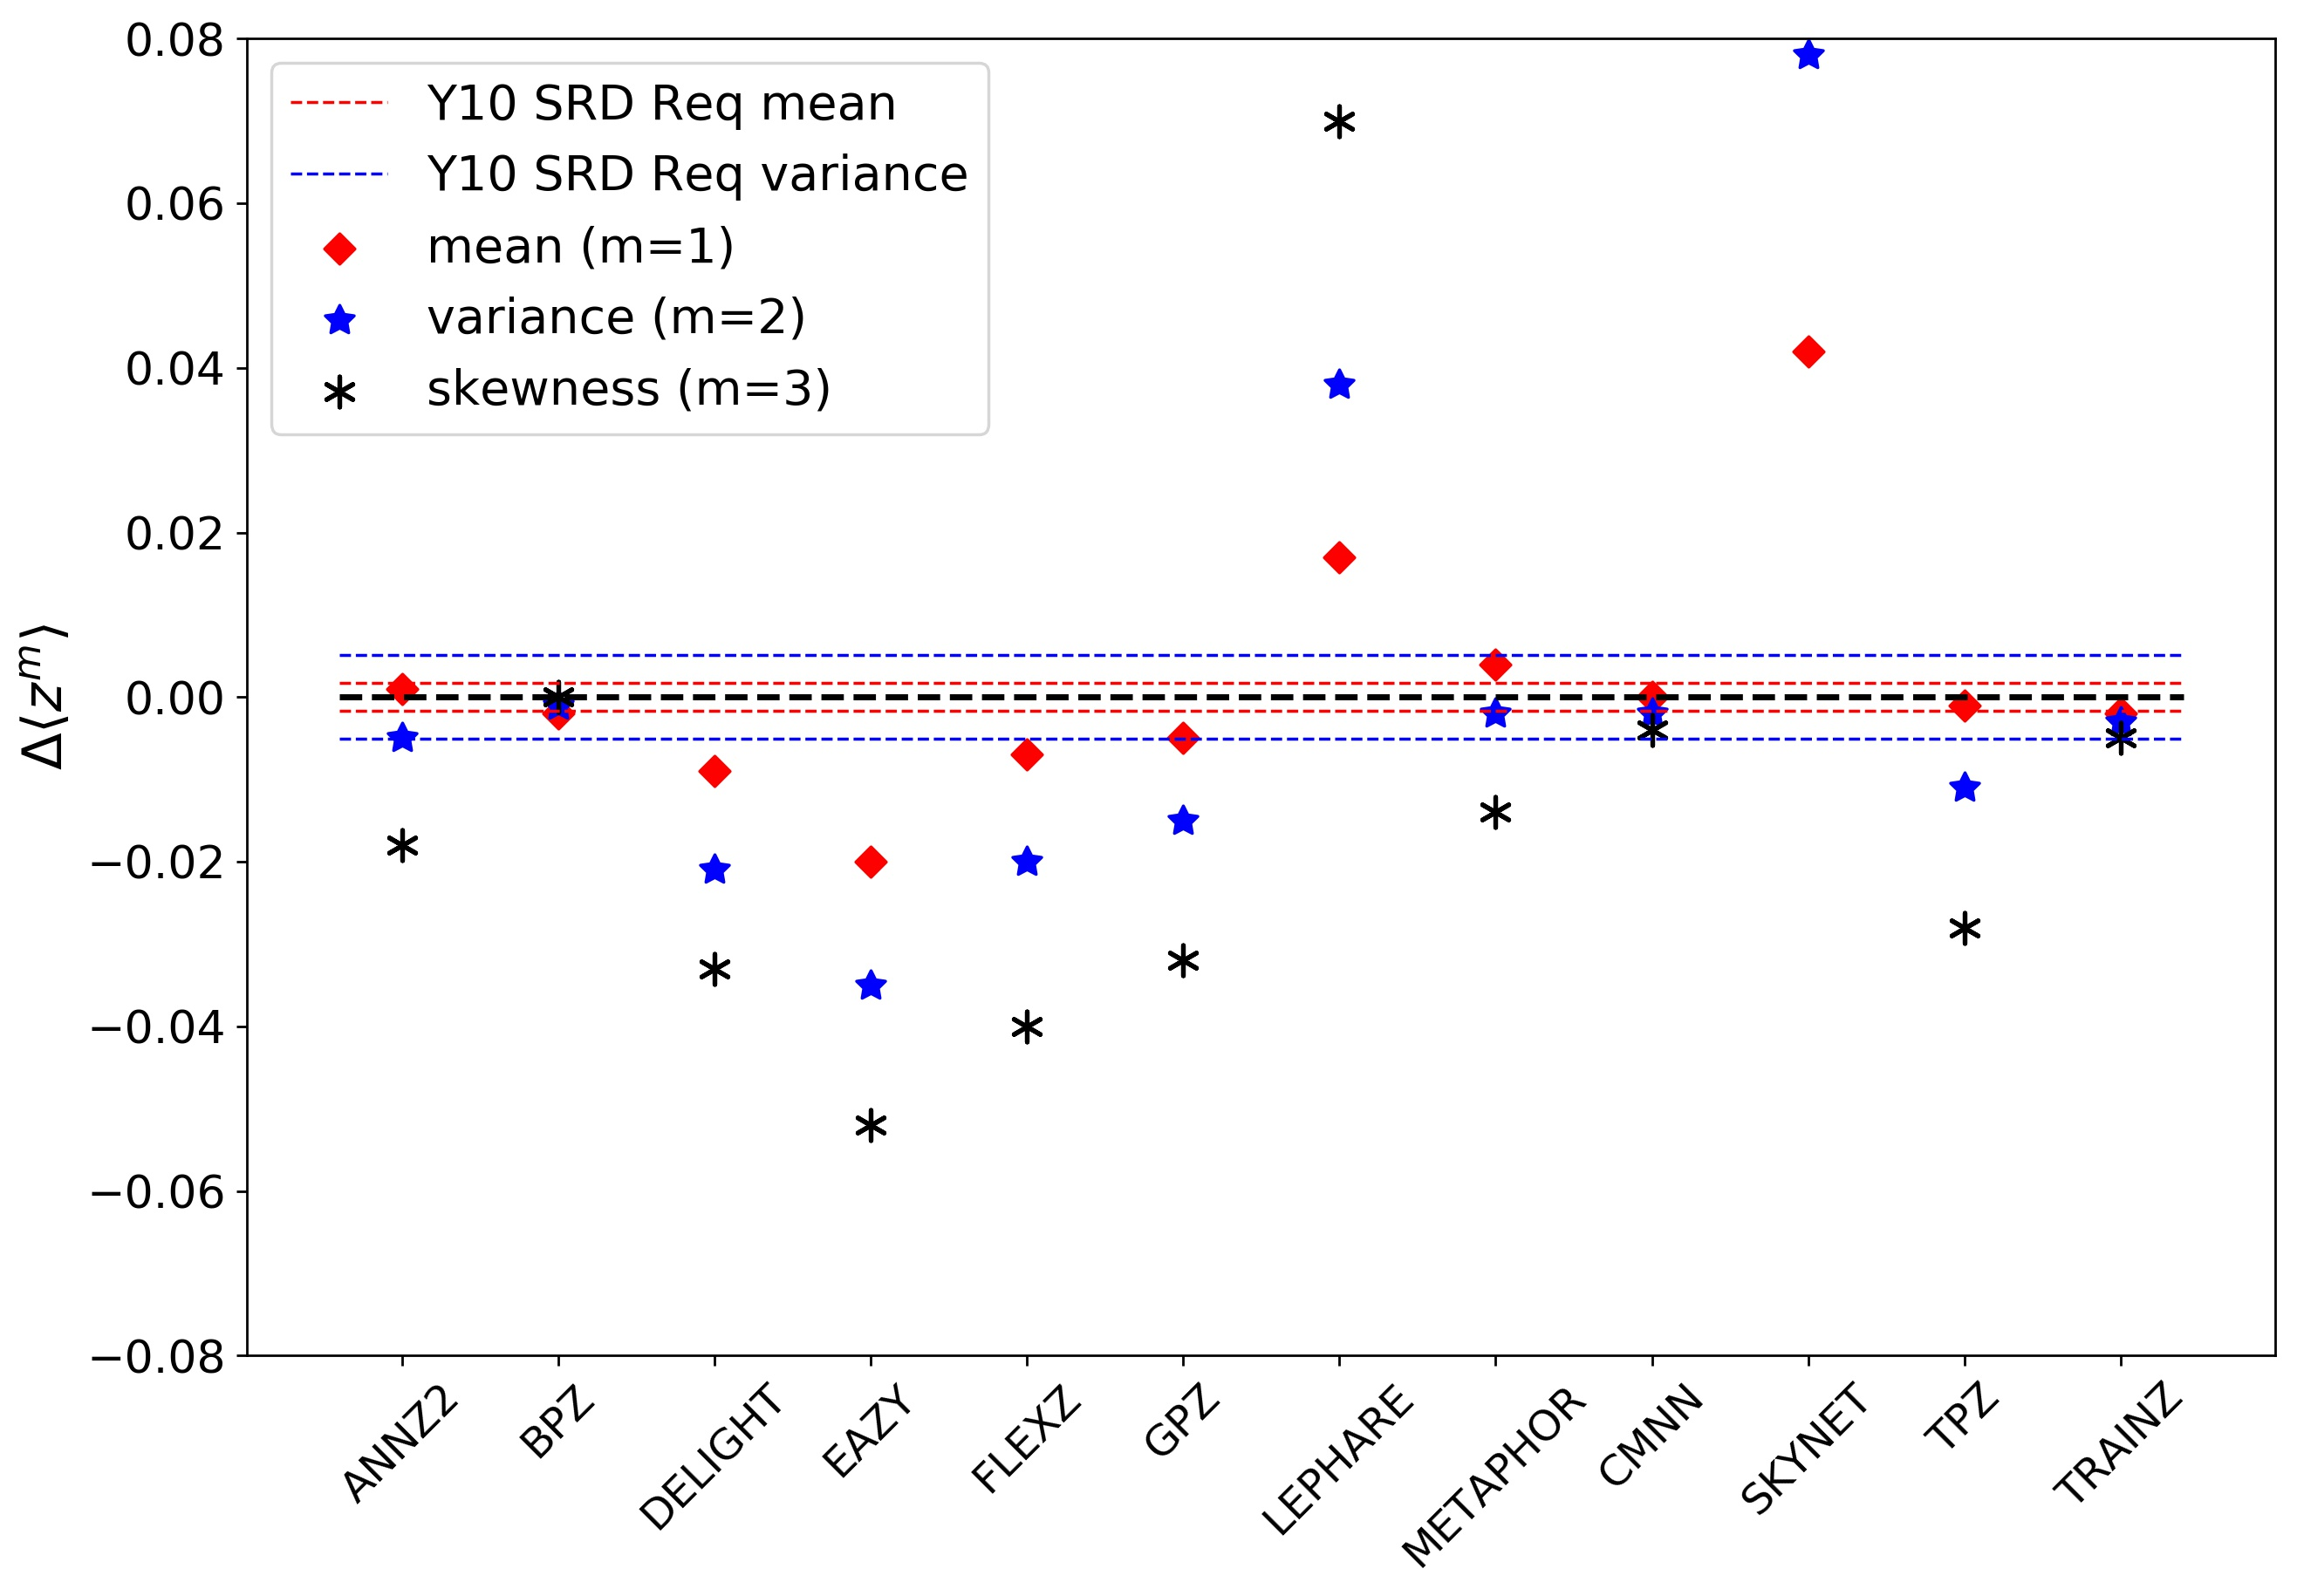
\includegraphics[width=0.75\textwidth]{fig/momentsplot_10yr.jpg}
\caption{Residuals of the first three moments of the stacked $\hat{N}(z)$ distribution.  Red and blue horizontal lines indicate the Year 10 DESC SRD requirements on accuracy of the mean and variance respectively.  Only a small number of codes are able to meet these specifications even with perfect training data.   }
\label{fig:moments}
\end{figure*}


We calculated the first three moments of the stacked $\hat{N}(z)$ distribution of all galaxies and compared it to the moments of the true redshift distribution.  Figure~\ref{fig:moments} shows the residuals of the moments for all codes.  Accuracy of the moments varies widely between codes, raising concerns about the propagation to cosmological analyses.  The DESC SRD \citep{Mandelbaum:2018} lists stringent requirements on how well the mean and variance of tomographic redshift bins must be known for each of the main DESC science cases.  We indicate the Year 10 (Y10) requirements assuming our true mean redshift of $z=0.701$ as dashed lines.  In this study with representative training data, \annz, \cmnn, \tpz, and our pathological \trainz\ estimator meet the Y10 requirement on the mean redshift.  Only \annz, \cmnn, and \trainz\ meet both requirements.  One should be concerned that many codes fail to meet this ambitious limit under perfect prior information because all codes are anticipated to do no better under realistically imperfect prior information, and indicates that additional calibration to remove these systematic offsets \citep[e.~g.~][]{Newman:2008} will likely be necessary in order to meet these stringent goals.


\skynet\ exhibits redshift bias in Figure~\ref{fig:nz} and is a clear outlier in the first moment of $\hat{N}(z)$ in Figure~\ref{fig:moments}.
The \skynet\ algorithm employs a random subsampling of the training set without testing that the subset is representative of the full population, and the implementation used here does not upweight rarer low- and high-redshift galaxies, as in \citet{Bonnett:15}, suggesting a possible cause that may be addressed in future work.

\section{\Pz\ point estimation and metrics}
\label{sec:pointmetrics}

While this work assumes that science applications value the information of the full \pzpdf, we present conventional metrics of \pz\ point estimates as a quick and dirty visual diagnostic tool and to facilitate direct comparisons to historical studies.

\subsection{Reduction of \pzpdf s to point estimates}
\label{sec:pointest}

Though we acknowledge that many of the codes can also return a native \pz\ point estimate, we put all codes on equal footing by considering two generic \pz\ point estimators, the mode $z_{PEAK}$ and main-peak-mean $z_{WEIGHT}$ \citep{Dahlen:13}, a weighted mean within the bounds of the main peak, as identified by the roots of $p(z) - 0.05 \times z_{PEAK}$.
Though $z_{WEIGHT}$ neglects information in a secondary peak of e.~g.~ a bimodal distribution, it avoids the pitfall of reducing the \pzpdf\ to a redshift between peaks where there is low probability.

\subsection{Metrics of \pz\ point estimates}
\label{sec:point_metrics}

We calculate the commonly used point estimate metrics of the overall intrinsic scatter, bias, and catastrophic outlier rate, defined in terms of the standard error $e_{z} \equiv (z_{PEAK} - z_{\mathrm{true}}) / (1 + z_{\mathrm{true}})$.
Because the standard deviation of the \pz\ residuals is sensitive to outliers, we define the scatter in terms of the Interquartile Range (IQR), the difference between the 75th and 25th percentiles of the distribution of $e_{z}$, imposing the scaling $\sigma_{\mathrm{IQR}} = \mathrm{IQR} / 1.349$ to ensure that the area within $\sigma_{\mathrm{IQR}}$ is the same as that within one standard deviation from a standard Normal distribution.
We also resist the effect of catastrophic outliers by defining the bias $b_{z}$ as the median rather than mean value of $e_{z}$.
The catastrophic outlier rate $f_{\mathrm{out}}$ is defined as the fraction of galaxies with $e_{z}$ greater than $\max(3 \sigma_{\mathrm{IQR}}, 0.06)$.

For reference, Section 3.8 of the \lsst\ Science Book \citep{Abell:09} uses the standard definitions of these parameters in requiring
\begin{itemize}
\item RMS scatter $\sigma < 0.02 (1 + z_{\mathrm{true}})$
\item bias $b_{z} < 0.003$ 
\item catastrophic outlier rate $f_{\mathrm{out}} < 10$ per cent 
\end{itemize}

\subsection{Comparison of \pz\ point estimate metrics}
\label{sec:pointmetrics_results}

Figure~\ref{fig:pz_pointestimates} shows \sout{both} point estimates \sout{both} $z_{PEAK}$ and $z_{WEIGHT}$ \boldblue{versus true redshift for all codes}.
Point density is shown with mixed contours to emphasize that most of the galaxies do fall close to the $z_{phot} = z_{spec}$ line, while points trace the details of the catastrophic outlier populations.

\begin{figure*}
\centering
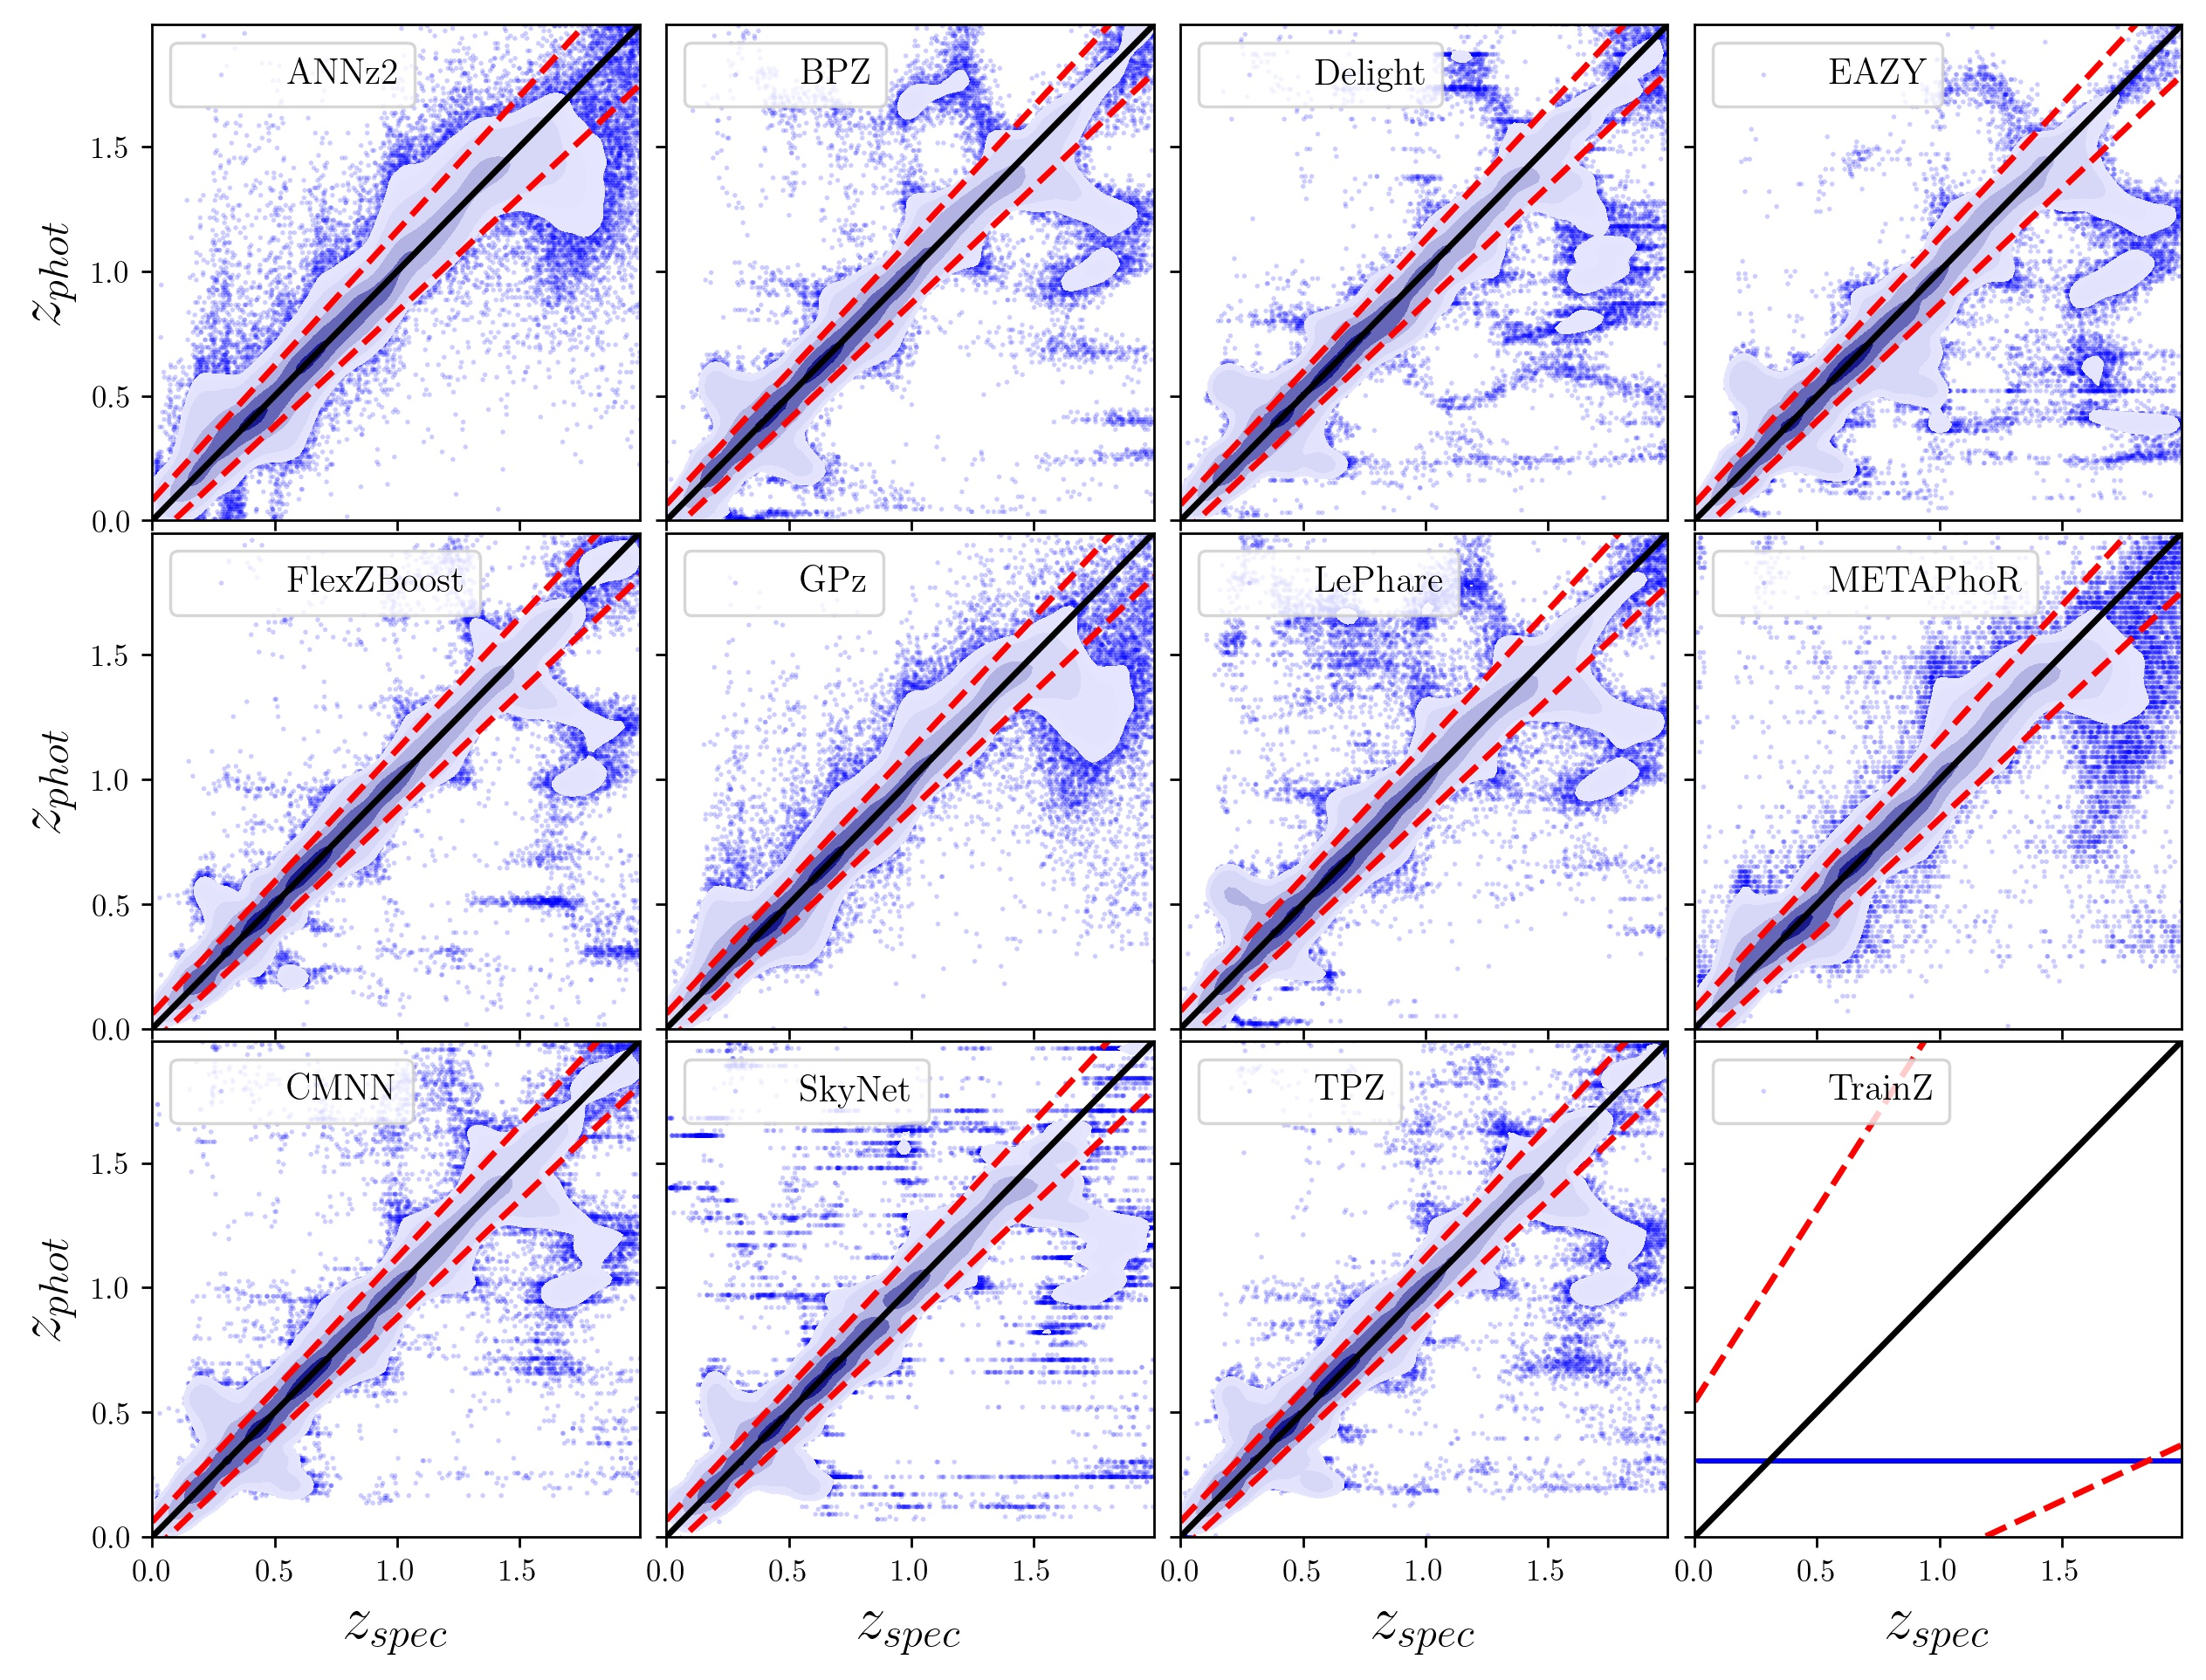
\includegraphics[width=0.49\textwidth]{fig/ZPEAK_szpz_threecolumn_12codes_navy_lowalpha.jpg}
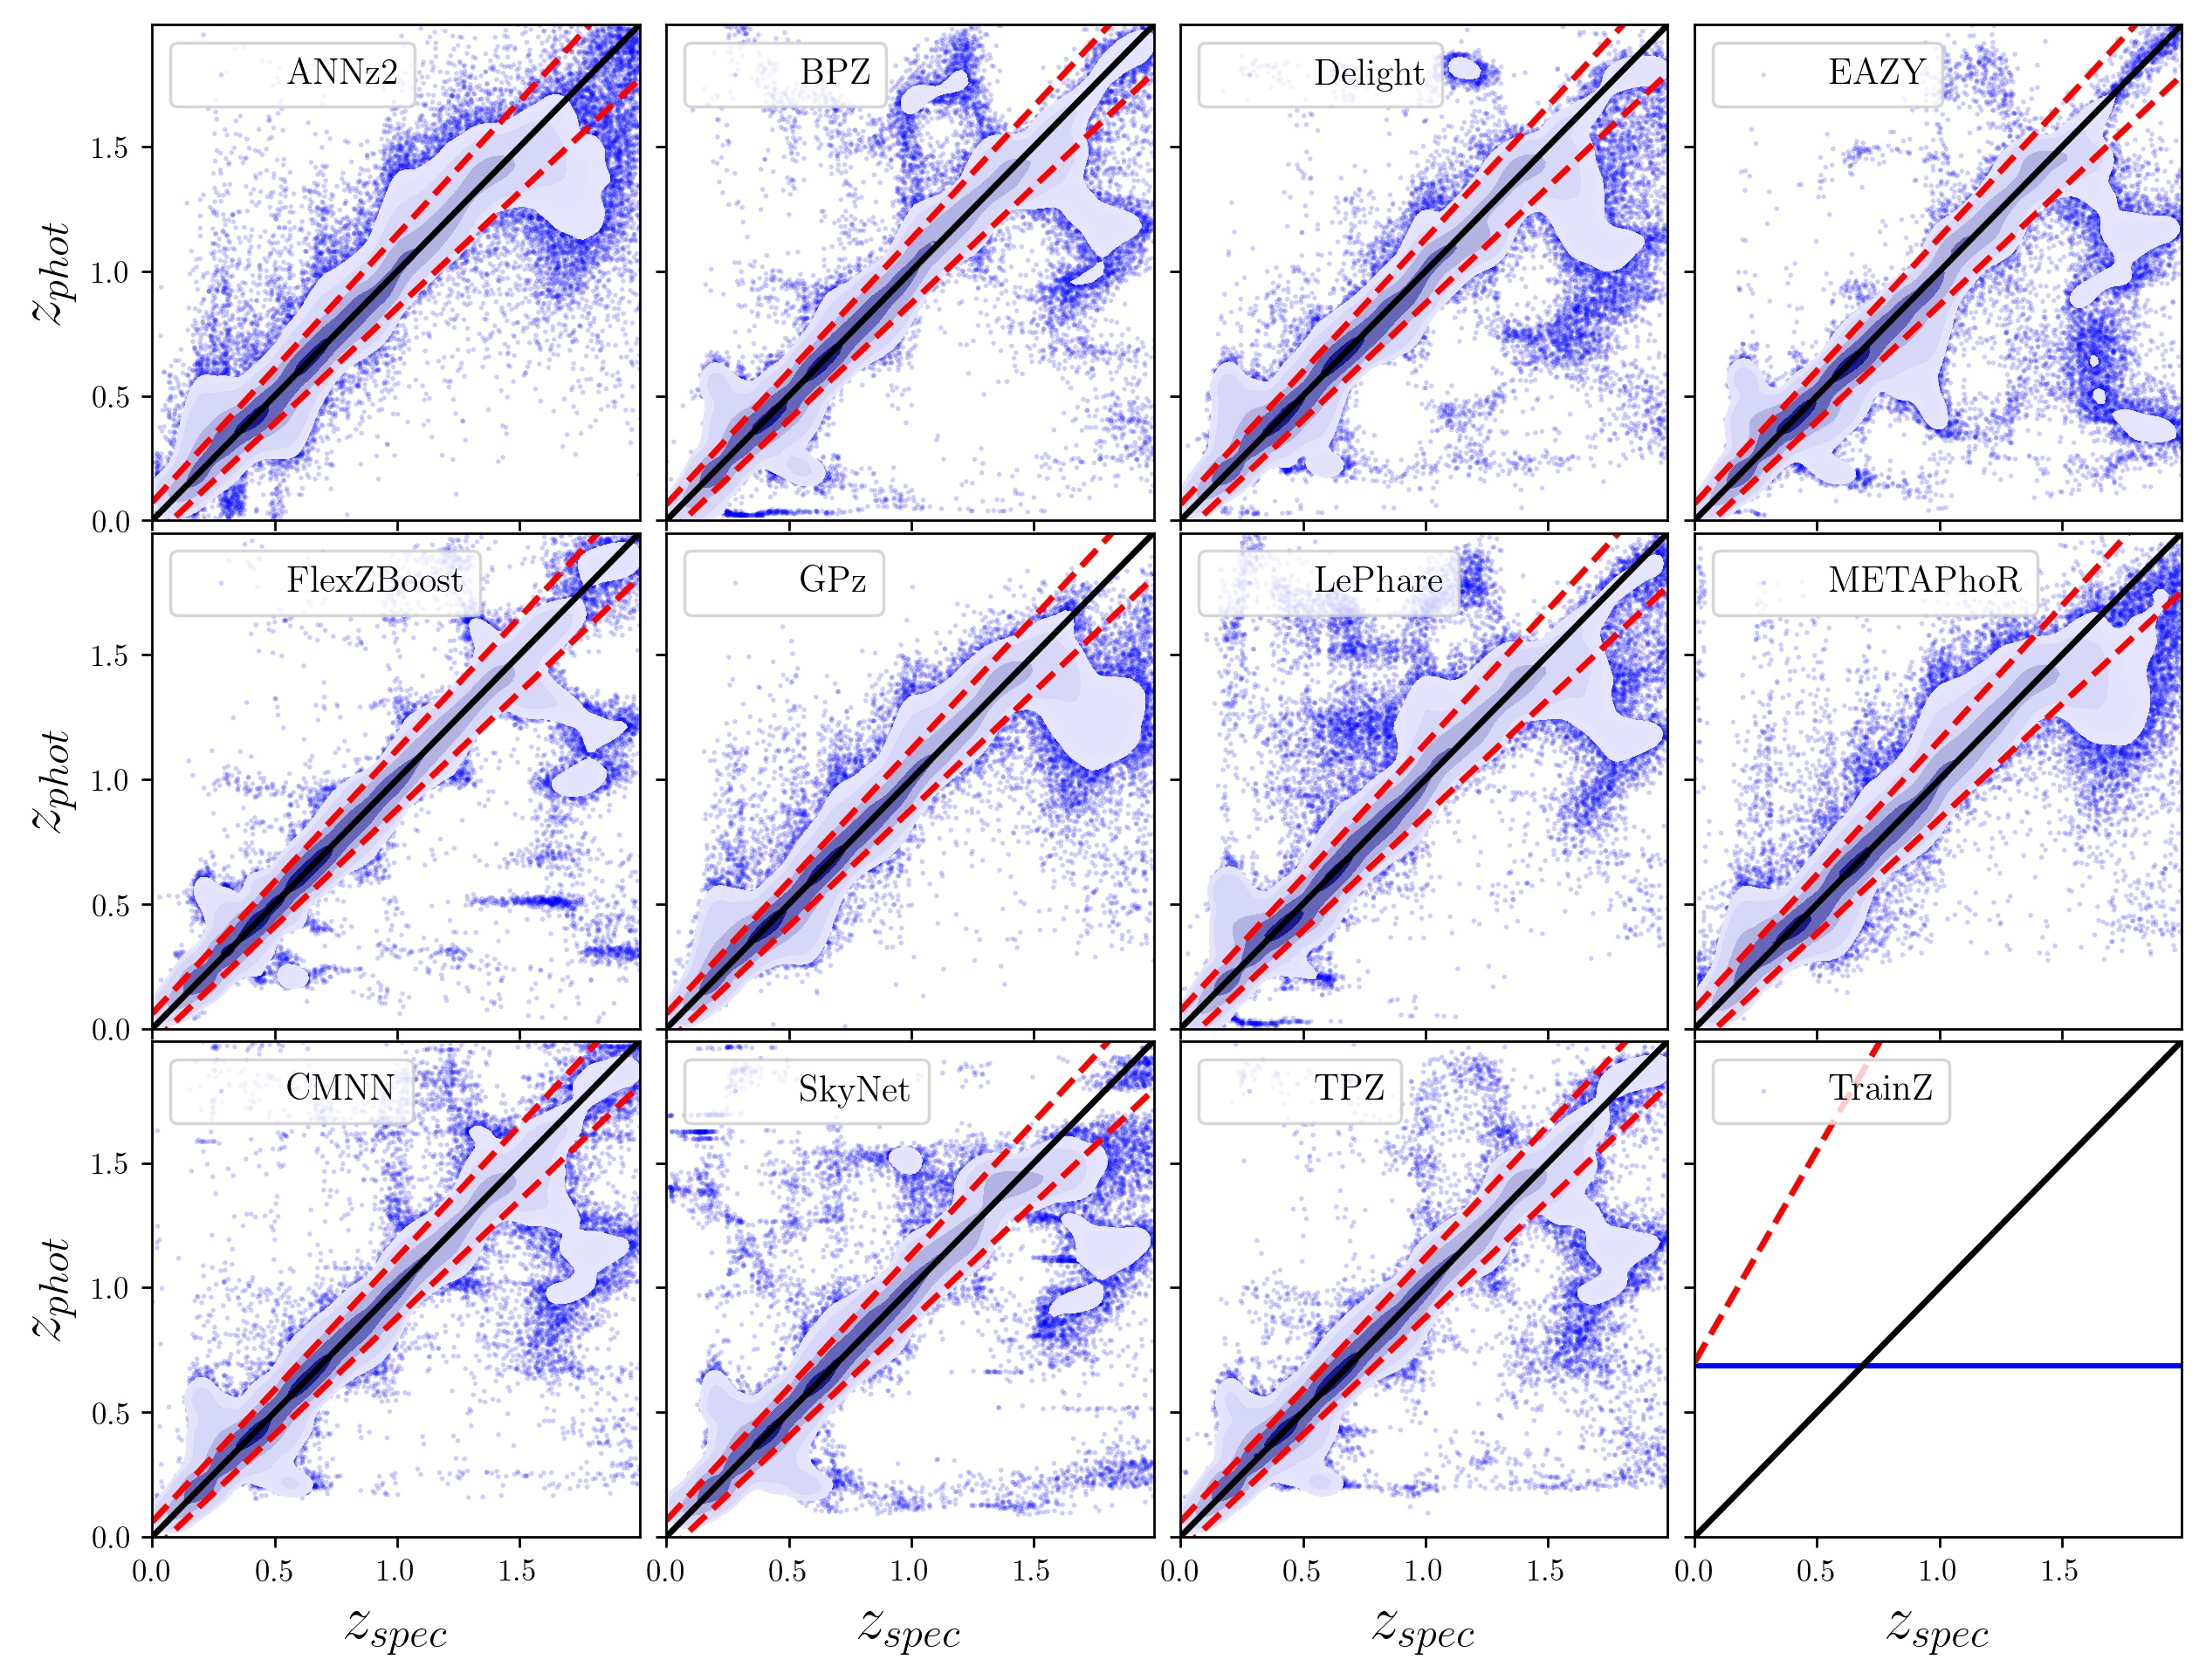
\includegraphics[width=0.49\textwidth]{fig/ZWEIGHT_szpz_threecolumn_12codes_navy_lowalpha.jpg}
\caption{The density of \pz\ point estimates (contours) reduced from the \pzpdf s with outliers (blue) beyond the outlier cutoff (red dashed lines), via the mode ($z_{PEAK}$, left panel) and main-peak-mean ($z_{WEIGHT}$, right panel).
The \trainz\ estimator (lower right sub-panels) has a shared $z_{PEAK}$ and $z_{WEIGHT}$ for the entire test set galaxy sample.}
\label{fig:pz_pointestimates}
\end{figure*}

The finite grid spacing of the \pzpdf s induces some discretization in $z_{PEAK}$.
The features perpendicular to the $z_{phot} = z_{spec}$ line are due to the $4000$ \AA\ break passing through the gaps between adjacent filters.  \boldblue{In the presence of genuine ambiguities in the colour space to redshift mapping, the compression of information down to a single number that is the point estimate redshift fails to adequately capture the more complex nature of the multimodal redshift matching: using the mode selects the highest peak while ignoring posterior probability in lower valued redshift peaks, while measuring the mean of a multimodal PDF often results in a value lying at a redshift between the peaks, removed from either/any of the most likely redshift solutions.  Thus,} \sout{E}even the strongest codes feature populations far from the $z_{phot} = z_{spec}$ line representing a \boldblue{genuine} degeneracy in the space of colours and redshifts.

\begin{table*}
\begin{center}
\caption{\Pz\ point estimate statistics}\label{tab:pointestimates}
\begin{tabular}{lcccccc}
\hline
\hline
                 &            & $Z_{PEAK}$  &          &  & $Z_{WEIGHT}$          &\\
\hline
\Pzpdf\ Code       & $\frac{\sigma_{IQR}}{(1+z)}$ & median  & \multicolumn{1}{|p{0.75cm}|}{\centering outlier \\fraction} & $\frac{\sigma_{IQR}}{(1+z)}$ & median & \multicolumn{1}{|p{0.75cm}|}{\centering outlier \\fraction}\\
\hline
\annz     & 0.0270  &  0.00063  & 0.044      & 0.0244  &  0.000307  & 0.047  \\
\bpz       & 0.0215  & -0.00175  & 0.035      & 0.0215  & -0.002005  & 0.032 \\
\delight   & 0.0212  & -0.00185  & 0.038      & 0.0216  & -0.002158  & 0.038 \\
\eazy      & 0.0225  & -0.00218  & 0.034      & 0.0226  & -0.003765  & 0.029 \\
\flexzboost& 0.0154  & -0.00027  & 0.020      & 0.0148  & -0.000211  & 0.017 \\
\gpz       & 0.0197  & -0.00000  & 0.052      & 0.0195  &  0.000113  & 0.051 \\
\lephare   & 0.0236  & -0.00161  & 0.058      & 0.0239  & -0.002007  & 0.056 \\
\metaphor  & 0.0264  &  0.00000  & 0.037      & 0.0262  &  0.001333  & 0.048 \\
\cmnn        & 0.0184  & -0.00132  & 0.035      & 0.0170  & -0.001049  & 0.034 \\
\skynet    & 0.0219  & -0.00167  & 0.036      & 0.0218  &  0.000174  & 0.037 \\
\tpz       & 0.0161  &  0.00309  & 0.033      & 0.0166  &  0.003048  & 0.031 \\
\hline
\trainz	   & 0.1808  &  -0.2086  & 0.000	  & 0.2335  & 0.022135  & 0.000\\
\end{tabular}
\end{center}
\end{table*}

The intrinsic scatter, bias, and catastrophic outlier rate are given in Table~\ref{tab:pointestimates}.
Perhaps unsurprisingly, performance under these metrics largely tracks that of the metrics of Section~\ref{sec:metrics} of the \pzpdf s from which the point estimates were derived.
All twelve codes perform at or near the goals of the \lsst\ Science Requirements Document\footnote{available at: \url{http://ls.st/srd}} and \citet{Graham:17}, which is encouraging if not unexpected for $i < 25.3$.

